\section{Research Plan}

\subsection{Automated Test Generation}
%\notetruong{We should update Figure 1 and relate this section to the steps in Figure 1.}
Automating application of advanced correctness methods to embedded systems framework-based code requires a twofold approach:

\begin{enumerate}
\item The automated production of \emph{test harness} code that allows modules or sets of modules representing ``units'' of system functionality to be tested using fuzzers or other tools, through the mediation of the DeepState tool.  This proposal is based on the idea of handling automated test generation via a layered approach.  The core is a tool that takes 1) source files and 2) a \emph{harness transform mapping} and outputs a DeepState harness.  The \emph{harness transform mapping} provides information on framework constructs, allowing the tool to read a source file and understand how a module to be tested acquires inputs and produces outputs.  This will include constraints provided by the framework that are more stringent than those of the C type system, and any framework-level specification of constraints on all modules producing outputs of a given type. For FPrime this will in part be tied to the notion of \emph{Ports}, which are used to communicate between \emph{Components}.  The semantics of such modules/components may vary between frameworks, however, so this specification will use a framework-independent language.  A harness transform mapping will be produced for every harness, and all harness generation work will be focused on the generic framework-independent representation.
\item The \emph{specification of correctness} will, for the most part, be pushed \emph{inside the implementation of the embedded system.}  Pushing specification to the harness level is fundamentally misguided unless absolutely necessary.  Specifications that engineers are likely to devised and that are checkable by current scalable analysis tools, whether dynamic or static, are almost always representable as \emph{runtime assertions} of some kind.  These assertions may be too expensive to use in deployed code, or in some forms of testing (e.g. realtime deadline testing) but should always be available for use in simulators and in isolated testing of individual components.  The C/C++ macro facilty and preprocessor make it easy to mark such code for removal.   This aspect of the project does not aim to simply encourage users to make use of e.g., C/C++ {\tt assert} facilities; rather, as discussed below, use of more advanced constructs is key to making specification more useful to testing tools.  In particular, this project emphasizes that while in some sense the distinction between assumptions and assertions (pre- and runtime/post- conditions) is not important for traditional testing, the distinction is critically important for efficient automated test generation that aims to avoid false positives.  Other specialized types of assertion include \emph{modifies} clauses.  We largely postpone the discussion of the specification side of the proposal until Section \ref{sec:modifies}, with the important exception that this proposal addresses \emph{preconditions} as relevant to harness-generation, rather than purely as runtime constraints.
\end{enumerate}

 \begin{figure}
   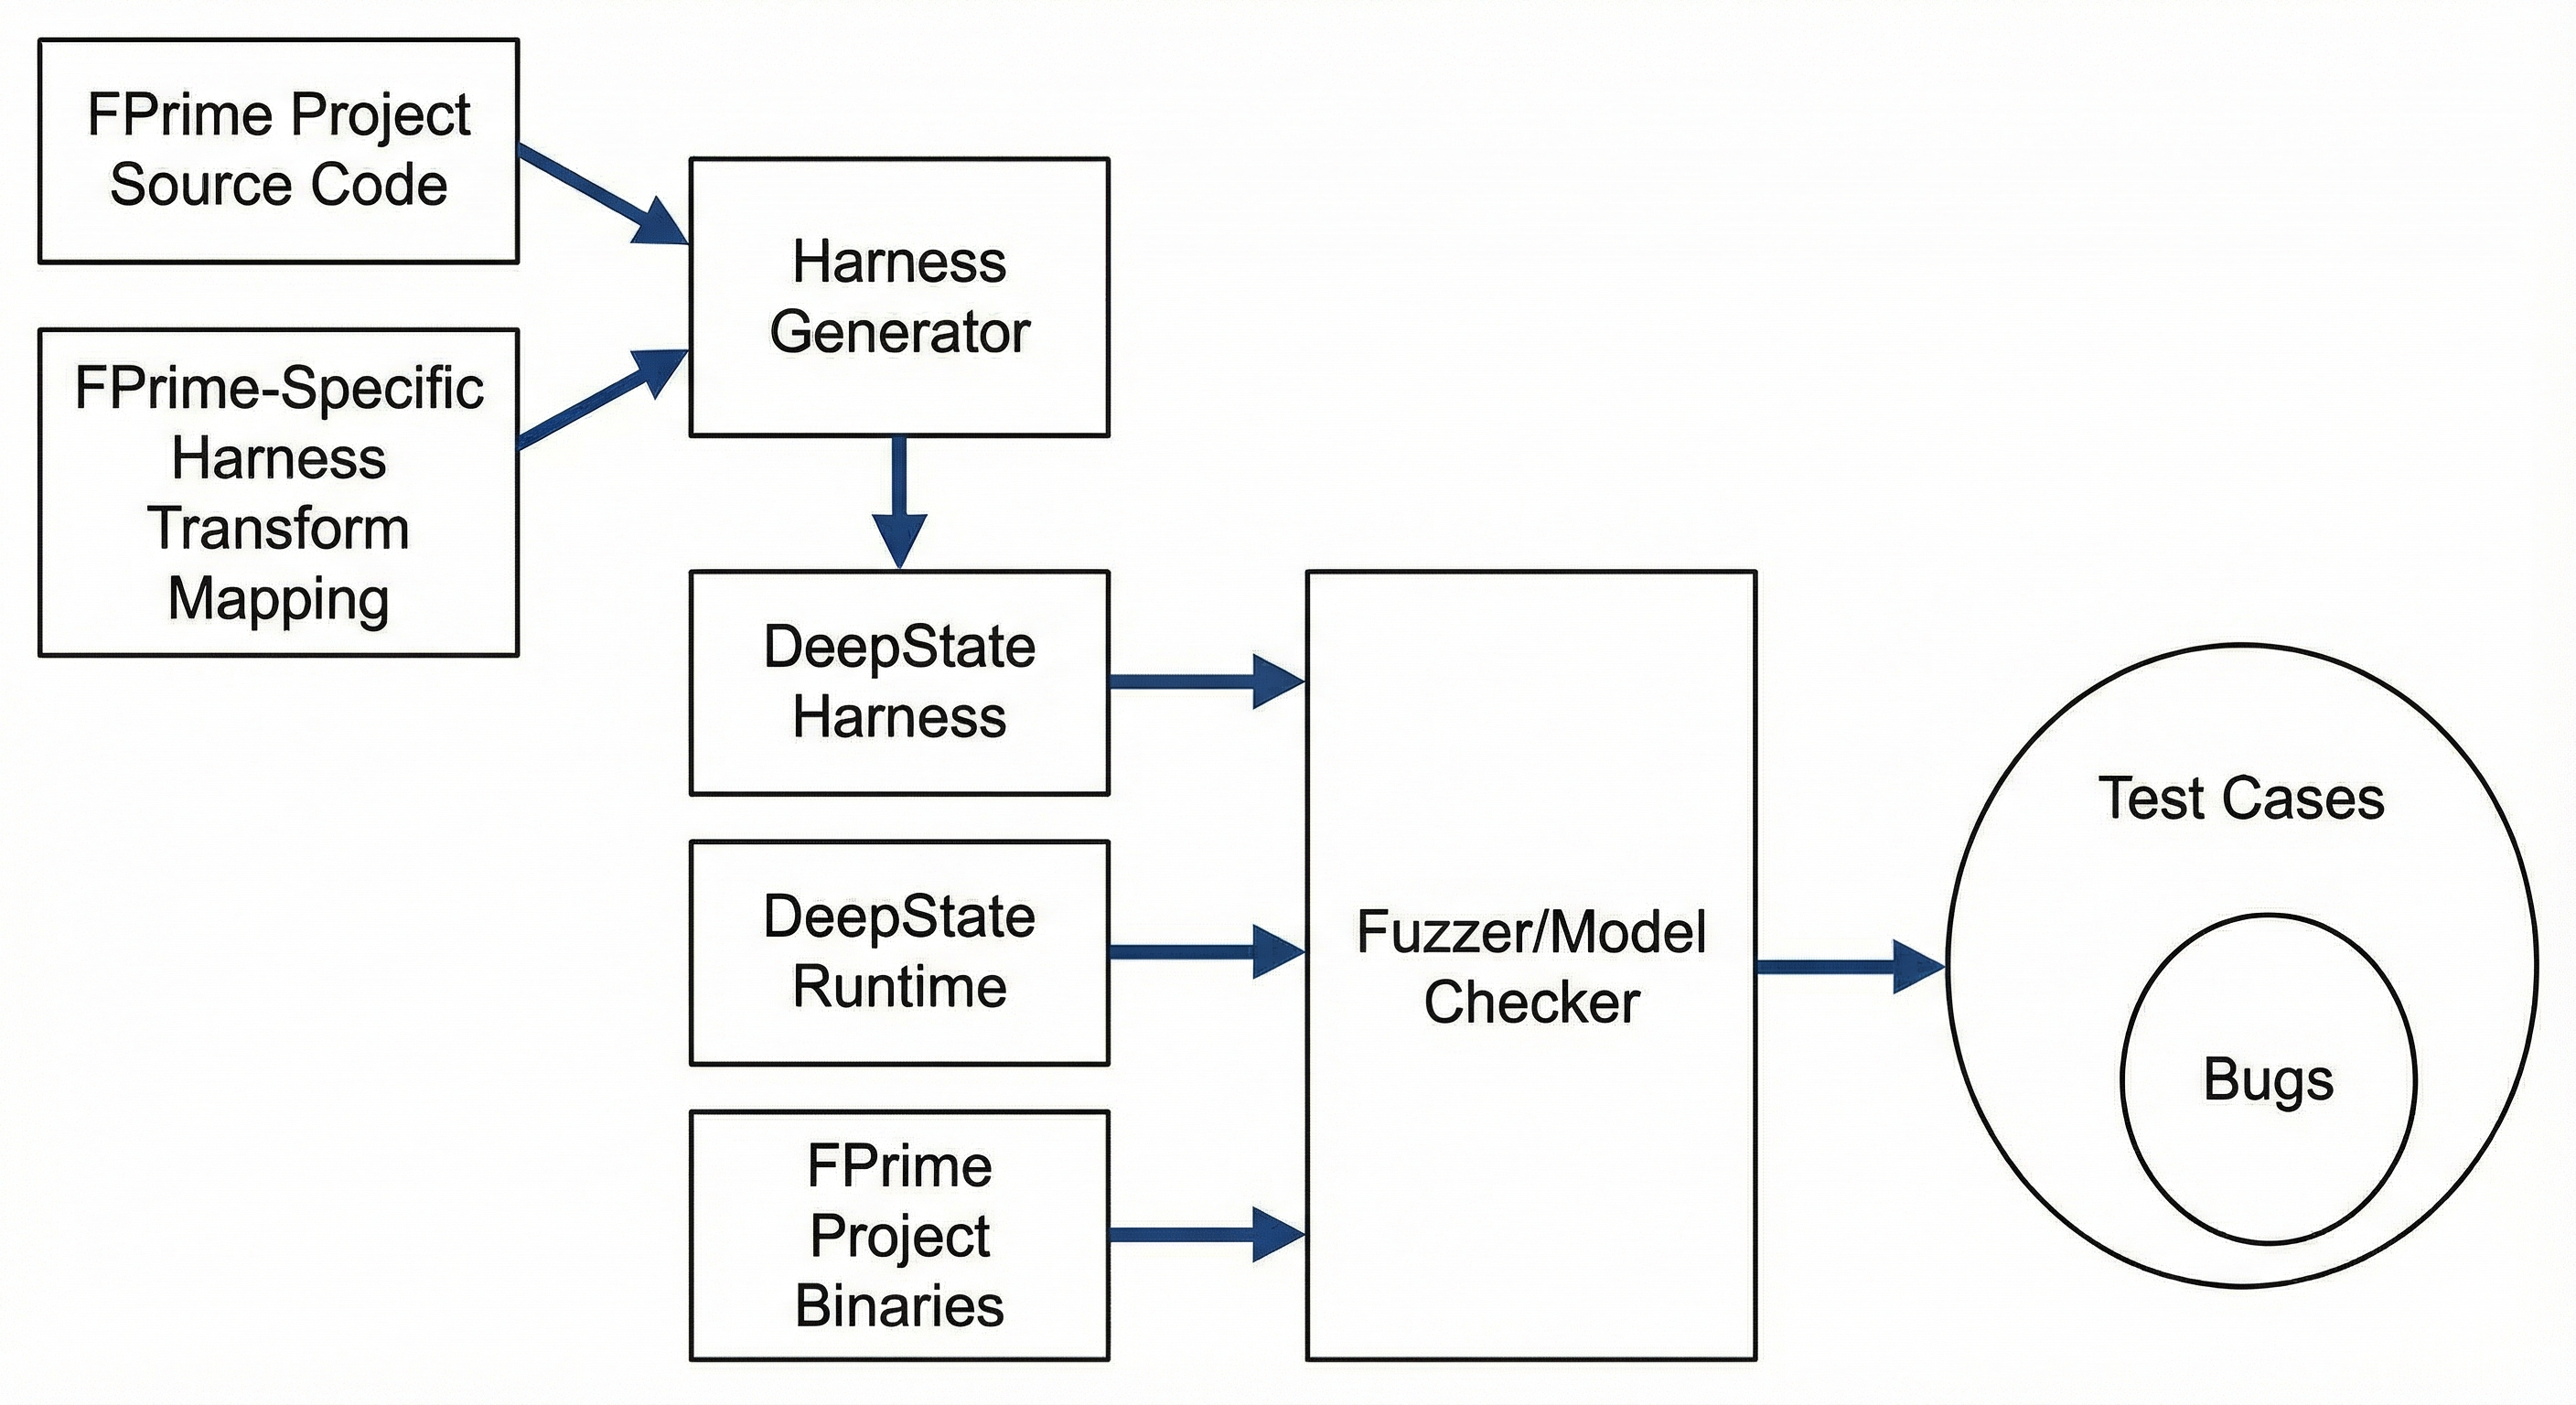
\includegraphics[width=\columnwidth]{overview.png}
   \label{fig:architecture}
   \caption{Overall Automated Test Generation Approach.  Note that specification is generally embedded in the FPrime source code, so it is available in other test environments, controlled by standard C/C++ DEBUG/TEST code omission controls for deployment/real-time testing environments.}
   \end{figure}

 Figure~\ref{fig:architecture} shows the overall design of the approach to test generation taken.  Given this overall approach, one obvious research challenge is the development of a harness transform mapping language and implementation that can apply to many embedded frameworks, and be extensible to other types of test generation problem.  We aim to address this by starting with FPrime but consulting exemplary programs using, e.g., AUTOSAR, in early design stages to ensure our approach generalizes. Beyond this fundamental challenge, we believe unanticipated challenges will be identified in the course of applying our approach to actual FPrime projects, including important open source NASA mission code.  This point applies not just to the harness generation stage, but to other aspects of the project described below; in each case we give examples of key challenges we believe have to be overcome with advances in dynamic analysis (powered by static analysis of framework-based code), but these are unlikely to be the only, or even most important challenges the project ends up addressing.
   
 Generating a test harness that understands the types input to a component is a relatively straightforward, if non-trivial, engineering problem, when the constraints of a framework map to input values in the C/C++ type system.  The DeepState system provides builtin generators for a large number of C and C++ types, including floating point values, and composing inputs from multiple port types, or tuple types, is easily handled by sequentially constructing values.   Handling real-world FPrime examples may require extending DeepState's generators to more complex array or C++ container types, but in general these transformations are simple (especially since FPrime provides serialization itself, which is basically what the DeepState type generators do, seriailzing raw byte streams from fuzzers into the entities code uses).  Similarly, the various types of FPrime component (active, passive, and queued) require only modest differences in DeepState instantiation.  Because DeepState supports strategies for input generation, such as forking concrete states for values too complex for symbolic execution using the {\tt Pump} construct, the translation must determine when such strategies are appropriate, and apply them, but in most cases a straightforward translation will suffice for fuzzing and model checking.

 However, in DeepState's context, in order to provide useful results to developers and make test generation efficient, we need to distinguish between {\tt ASSUME} failures (invalid tests) and {\tt ASSERT} failures (bugs).   This is not a distinction particular to DeepState, though most programming languages do not make any distinction between {\tt assert} representing a pre-condition and {\tt assert} representing a bug.  This is natural; assertion facilities were designed for use in running an entire program, where a failure to satisfy a checked precondition is a bug, just like any other assertion failure.  But in testing isolated pieces of code, this is not true; a unit test is not interesting if it violates a unit's preconditon, since these are the responsibility of the calling context.  Similarly, preconditions on port values are to be established by interfacing components in FPrime.  In these contexts, a failed assumption should 1) be avoided if possible at the stage of generation of values and 2) when this is not possible, failures of assumptions, unlike other {\tt assert}s should \emph{not} be reported to a user.

 In some cases, however, checking a single component in isolation may not be an effective way to detect faults; only a sequence equivalent to a set of API calls can expose a problem in a system (e.g., that a components produce a global state that causes another component to violate an invariant); this may be essentially equivalent to taking threaded component interactions and transforming them into sequential behavior, to make behavior reproducible by a fuzzer.   Moreover, even in cases where the violation of a specification can, in theory, be discovered without calling multiple functions, the state space may be too large to explore with a fuzzer or symbolic execution tool.  In such cases, exploring only states produced by valid ``call sequences'' has two benefits:  first, the space itself may be much smaller, and easier to explore, than the full set of possible input values.  Second, errors in this part of the input space are more important.  Even if a precondition is not sufficiently restrictive to guarantee correct behavior, if the ``bad'' inputs are never, in practice, generated by the functions that modify system state, the fault may not matter.  In cases where constructing a sufficiently exact precondition is difficult for engineers, such ``in-use'' verification may be the only avenue to system assurance.  We propose to let users annotate \emph{sets} of components to be tested as an API-call-sequence group, extending recent work exploring this concept~\cite{blatter2018static,MetAcsl}.  A key point is that \emph{in these testing scenarios} precondition failures, except on the first-activated component in a sequences, \emph{are} actual bugs, since the bad data results not from a test-input generator like a fuzzer, but from the behavior of system components acting on valid inputs.
 
\begin{figure}[t]
  \hspace{-12pt}
  \begin{subfigure}{0.492\columnwidth}
  {\scriptsize
  \begin{code}
void update\_state(struct state\_t *s, uint64\_t bv) \{
  ASSUME(valid\_state(s));
  ASSUME(valid\_bv(bv));
  ...
\}

void process\_both\_sensor\_readings(struct state\_t *s) \{
  ASSUME(valid\_state(s)); 
  unit64\_t s1\_bv = acquire\_s1(), s2\_bv = acquire\_s2();   
  update\_state(s, s1\_bv);  update\_state(s, s2\_bv);  
\}
  
void process\_one\_sensor\_reading(struct state\_t *s) \{
  ASSUME(valid\_state(s)); 
  unit64\_t s1\_bv = acquire\_s1(); 
  update\_state(s, s1\_bv); 
\}
\end{code}
}
\end{subfigure}
\begin{subfigure}{0.492\columnwidth}
{\scriptsize
\begin{code}
struct state\_t *NewState() \{
  return DeepState\_Malloc(sizeof(struct state\_t));   
\}
    
TEST(SensorReading, UpdateNeverSlow) \{
  struct state\_t *s = NewState();
  DeepState\_Timeout(
    [\&]\{update\_state(s, DeepState\_UInt64());\},
    MAX\_EXPECTED\_UPDATE\_TIME);
\}

TEST(SensorReading, AvoidCrashes) \{
  struct state\_t *s = NewState();
  for(int i = 0; i < TEST\_LENGTH; i++) \{
    OneOf(
        [\&]\{process\_both\_sensor\_readings(s);\},
        [\&]\{process\_one\_sensor\_reading(s);\});
  \}
\} 
\end{code}
}
\end{subfigure}
  \caption{Sensor reading code and DeepState test harness}
  \label{fig:assumption}
  \end{figure}

These concerns require significant advances in several areas of dynamic analysis: first, a complete and principled approach to the problem of handling pre-conditions/assumption semantics, and second, an investigation of how to let fuzzers take advantage of the significant additional structure provided by property-based testing, including such assumptions.  Consider the code in Figure~\ref{fig:assumption} (abstracted away from FPrime details, in order to make the underlying issue, which is not limited to embedded systems frameworks, clear).  This defines two different tests of software that reads sensor values and incorporates them into a system state.  The two tests check two different properties:  {\tt UpdateNeverSlow} ensures that updating the sensor is never too slow.  It is checked, potentially, over \emph{all} valid inputs, not just ones produced by the actual sensor reading code in {\tt acquire\_s1} and {\tt acquire\_s2}.  The second test, {\tt AvoidCrashes} starts the system up in some valid state, and repeatedly either reads both sensors or only sensor one.  There is no explicit property, only the expectation that the system will not crash; tests can be executed using LLVM sanitizers to check for integer overflow and other undefined behavior.  Generating such harnesses automatically is a significant challenge, but our research agenda also includes solving problems that would appear even for manually produced harnesses.  For example, what is the proper semantics of the {\tt ASSUME} in {\tt update\_state}?  It depends on the test.  In {\tt UpdateNeverSlow}, a fuzzer will often generate an input value that violates the (possibly complex) requirements on valid states and sensor readings.  These invalid inputs should not be flagged as bugs (the default behavior of most implementations of {\tt ASSUME}), but instead the test should be \emph{abandoned} without indicating that it failed.  However, in {\tt AvoidCrashes}, since we are not directly generating state values and thus, {\tt update\_state} is not an \emph{entry point} for the test, assumption violations \emph{should} result in failed tests.  We aim to synthesize code to make assumptions automatically take on the proper semantics during test execution (including symbolic execution using constraint solvers).

This point about preconditions/{\tt ASSUME} brings up a second point.  Preconditions, when they have an {\tt ASSUME} semantics, are fundamentally different than other branches in code.  A fuzzer will attempt to explore the behavior of branches in {\tt valid\_state} and {\tt valid\_bv} just as it explores branches in {\tt update\_state} or {\tt acquire}.  However, it is often possible to enumerate a vast number of paths that differentiate only invalid inputs, and so produce very little real testing.  A classic example is ``testing'' a file system by producing a huge variety of unmountable file system images, rather than actually executing POSIX operations~\cite{CFV08,AMAI}.  In previous work at NASA, on the Curiosity Rover file system, we determined that it was almost impossible to find bugs in the system using symbolic execution or explicit-state model checking if we allowed the system to devote too many resources to exploring mount semantics that did not result in a viable file system.

DeepState's harness specification language extends its GoogleTest basis to explicitly mark {\tt ASSUMEs} and indicate which branches are pre-conditions, and so can help avoid this problem.  In some fuzzers, this means prioritizing inputs to mutate based on whether they execute any code other than validity checks; but in fuzzers, such as Angora~\cite{angora} and Eclipser~\cite{eclipser}, that use lightweight constraint-solving to cover branches, the process can be more sophisticated.  We have begun discussions with the Eclipser team, and they confirm that identifying precondition code and devising suitable heuristics to handle it (e.g., never solve for a negation of a passed check) should improve performance.  Fuzzing of individual functions or sets of functions is a highly promising area: most fuzzing is applied at the whole-program level, where input generation can simply be too hard.  By focusing on a middle-ground between unit testing and whole-program fuzzing, essentially using fuzzer technology to drive property-driven testing at the function/FPrime component level, the problem is made tractable.  Prioritizing paths that include more than just input validation is an explicit goal of, e.g., AFLFast~\cite{aflfast}, but it must work with an implicit definition based on path frequencies, while we have access to ground truth.  Given the complexity of state validity checks, there may be hard-to-reach, but uninteresting, ways to create invalid input; AFLFast will \emph{prioritize} such paths, while we will (correctly) avoid them.

However, it is possible to be more aggressive with preconditions that flow directly from the test harness to a function, especially known, repeated preconditions established by framework semantics.  Namely, in a large number of cases, it is possible to \emph{actually produce values satisfying a precondition from a fuzzer-chosen value} rather than simply abort the run.  This does not violate the semantics of the SUT; it merely transforms one arbitrary input into another, with a fixed mapping so that the fuzzer can still learn from the pattern of inputs, \emph{as transformed}.  Consider the simple case of ranges.  If a component's code begins with {\tt ASSUME ((input > 10) and (input < 256))} where {\tt input} is an integer parameter to the function, or if a framework allows specification of such ranges on its version of ports, and this assumption takes place before any assignments to {\tt input} (which will always be the case with input ports), then we can replace the assumption with the code:

  {\tt if ((input <= 10) || (input >= 256)) input = (abs(input) \% 245) + 11}

Rather than testing if {\tt input} is in a range, this simply maps values that violate the assumption into valid values, that could have been provided by the fuzzer.  In such simple cases, of course, the developer of the test harness could have written {\tt DeepState\_IntInRange(11, 245))}but when the values in an assumption are dynamically computed inside the called function and/or involve state values not visible to the test harness, or are more complex than a simple range check, this is often impractical.   Moreover, forcing users to think about such problems violates the principle of making automated test generation a seamless part of the development environment, supported by fully automated harness generation. We propose to provide forms of {\tt ASSUME} that enable automatic mapping of inputs, without developer action (other than using our variants of ASSUME), using a mix of guaranteed transformations such as in the range case and ``search-based'' approaches that find a nearby value of an input that satisfies an assumption (particularly useful in case of, e.g., parity checks).

As far as we are aware, the problem of mapping inputs (rather than producing inputs) to satisfy a predicate has not been explored in the literature.  Note that a ``mapping'' may in the most general case be a \emph{search}: while also amenable to a solution like that above, a parity check can be satisfied simply by incrementing a fuzzer input byte until it satisfies a check.  This most-general approach may be useful in some cases, such as complex checksums with a small size, where a complete solution cannot be produced.  On average the time to produce a 16 bit checksum by brute force search from random bytes, for example, may be an acceptable overhead to fuzzing.
 We note that this approach to preconditions is not limited to DeepState and/or embedded systems; a manual transformation of this sort is given as essential advice for users of the Echidna smart-contract fuzzer \cite{echidna-advice}.  However, while Trail of Bits even provides an API for the simple range case, the complexity of correctly using the shift from assumption to mapping is such that it is seldom done for more complex cases.
  
 This effort also connects to a second fuzzing research thrust: making specification elements that do not correspond to simple code coverage visible to a fuzzer.  In this example, consider the {\tt DeepState\_Timeout} check (note that this itself is functionality we will develop as part of handing timing constraints in DeepState).  Unless we break down the timing analysis explicitly using a set of conditional branches, coverage-driven fuzzers cannot distinguish an execution that is very slow (close to violating the constraint) from one that has the minimum execution time possible.  We propose to make timing of such specified events visible to a fuzzer, by modifying coverage bit-vectors to incorporate bucketing of execution time.  Once we add such novel coverage measures, and introduce distinctions between coverage classes (as with preconditions), we will research how to balance competing priorities in more complex notions of coverage.  In addition to implicit execution properties such as timing, this can apply to coverage of data structures, for fuzzing data-driven code such as machine-learning algorithms, where much behavior is implicit, e.g., the route taken through a forest of decision trees.  In general we aim to extend the work~\cite{aflfast,lemieux2018fairfuzz,vuzzer,zhao2019send,aschermann2019redqueen}, that prioritizes certain program paths in an intelligent way, by exploiting more specifcation constructs that developers embed in code.


% Additionally, in some cases, checking a single function may not be an effective way to detect faults; only a sequence of API calls can expose a problem in a system (e.g., that a function produce a state that causes another function to violate an invariant).  \acsl annotations provide enough information for a fully-automated translation to a harness enabling dynamic analysis in the case of proving properties of a single function, but this is no longer true for groups of functions.  Moreover, even in cases where the violation of a specification can, in theory, be discovered without calling multiple functions, the state space described by the precondition for a function may be too large to explore with a fuzzer or symbolic execution tool.  In such cases, exploring the space described by valid calls of other functions has two benefits:  first, the space described by a sequence of calls may be much smaller, and easier to explore, than the full set of possible input values to a function.  Second, errors in this portion of the input space are more clearly realistic scenarios.  Even if a precondition is not sufficiently restrictive to guarantee correct behavior, if the ``bad'' inputs are never, in practice, generated by the functions that modify system state, the fault may never appear in practice.  In cases where constructing a sufficiently exact precondition is difficult for engineers, such ``in-use'' verification may be the only avenue to system assurance; proof is impossible without a restrictive enough precondition, and dynamic methods may scale very poorly to, e.g., a large unstructured byte buffer such as a hash table.

% In principle, of course, users can write a new function (a kind of ``ghost function'' not really executed---in practice, a test harness) expressing the desired mix of API calls that preserve an invariant; however, this is a serious burden on a user, and users are likely to make errors in this task~\cite{CFV08,AMAI,scriptstospecs,groce2015verified,groce2018verified}; we instead propose to let users annotate (in an extension of \acsl) sets of functions to be tested as an API-call-sequence group.  E.g., annotating a set of file system functions ({\tt mkdir}, {\tt rmdir}, {\tt readdir}, etc.) as such a group could allow the automatic generation of a DeepState harness that checks for cases where a sequence of valid function calls can violate a precondition or cause a fault despite preconditions being satisfied.


%%% Local Variables:
%%% mode: latex
%%% TeX-master: "main"
%%% End:


\subsection{Automated Specification Checking}
\label{sec:modifies}

\emph{Modifies clauses}~\cite{Meyer1997OOSC,GuttagHorningWing1985Larch} are used to specify which memory locations a function can alter; they have been used in languages since Larch and are a core feature of modern verified languages such as Dafny~\cite{Dafny}.  Modifies clauses are a natural fit for incorporation into the FPrime framework, since FPrime generally encourages developers to avoid dynamic memory allocation after system initialization if at all possible, and in the circumstances where it is required, to make use of the included buffer manager pattern.  This means that the intended memory usage of every function is generally much easier to determine than with typical C++ software.  While FPrime offers guidelines and patterns to reduce the risk of languages such as C and C++ that do not provide memory safety guarantees, those risks remain present.  In the case of FPrime, 

In previous work at NASA JPL, PI Groce made it possible to check modifies clauses for C programs, including in the context of explicit-state model checking~\cite{vmcai08}.  That work relied on the CIL (C Intermediate Language) framework, which is limited to C programs and is now deprecated.  In this proposal, in order to show how frameworks can be exploited to provide sophisticated checking for properties, embedded in the source code for a system, an LLVM-pass based equivalent will be developed, providing a way to dynamically establish a set of memory boundaries computed at runtime, and check every memory write (and potentially some reads) for inclusion in the allowed locations.

The proposed work extends the original CIL-based approach in several critical ways. First, the checkable set
of memory locations to be established for each function via API calls will be derived from
FPrime’s component metadata: port definitions, buffer allocations, queue depths, and topology wiring all serve
to define \emph{intended} aliasing and ownership relationships. These will be synthesized automatically into runtime region boundaries for developers to use in the source code. Second, because components often
interact through message buffers whose layout is generated from FPP models, the pass will leverage that
generated structure as an authoritative description of which bytes are permissible for a given
operation. Third, the LLVM instrumentation will support two distinct modes: a debugging mode that eagerly
checks every write, producing immediate diagnostic traces, and a fuzzing-optimized mode that coalesces
repeated checks and integrates with sanitizers (e.g., ASan) to minimize performance overhead for fuzzing.  

Finally, to remain consistent with DeepState’s semantics for assumptions and assertions, modify-clause
violations will be treated in a manner parallel to runtime assertion failures. When the violation arises from
invalid fuzzer-generated inputs, i.e., when a precondition is unsatisfied, the system can suppress the report. But when a violation occurs on a path reachable from a valid harness entry point,
the error will be reported as a true bug. This distinction is essential for embedded developers, whose systems
must avoid memory corruption even in the presence of complex component interactions.  The result will be
the first demonstration of practical, runtime-enforceable modifies-clause checking for framework-based C++
embedded systems, and a model for using framework semantics to lift verification mechanisms beyond their
traditional language-centric formulations.  Moreover, to our knowledge no dynamically configurable runtime checking for modified clauses is available at present, and while requiring more user input and expertise, this work will add to the set of LLVM sanitizers in a powerful way that will be useful beyond the FPrime or embedded community.

Exploring how to make modifies clauses usable and lightweight for developers will help us determine the space of possible additonal runtime checks to implement, and how FPrime or other frameworks can bridge usability gaps by automatically producing reliable annotations for users.  A model for our approach is the ACSL~\cite{ACSL} runtime assertion tooling for the Frama-C analysis framework~\cite{KKP2015:FAC} , though we aim to provide a more developer-friendly approach that leverages embedded frameworks and FPP models to automate annotation, to fully integrate with fuzzers and test generation tools, and to handle C++ (which is handled in a very limited way in Frama-C at present; for instance, modifies/assigns clauses cannot be checked in C++ code) fully.

\subsection{Framework Aware Mutation Analysis}

Mutation analysis provides a quantitative measure of test adequacy by introducing small, syntactic changes (which are likely to change the semantics for the worst, thus serve as ``artificial bugs'') into a program and evaluating whether the existing tests detect the injected faults.
Traditional mutation testing tools operate primarily at the source level, applying generic syntactic
operators such as arithmetic replacement, logical negation, or constant modification. While effective
for many domains, such operators do not reflect important fault classes in embedded systems
frameworks, where a substantial fragment of the system’s semantics resides in architectural structure rather than in
individual expressions.

In frameworks such as FPrime, consequential defects often arise from subtle deviations in
configuration or interaction patterns: mis-wired ports, altered queue depths, changed command or
telemetry dictionaries, or incorrect initialization sequencing. These errors are difficult to express
using conventional mutation operators but correspond closely to real failures observed in deployed
embedded systems. This motivates the development of \emph{framework-aware mutation operators},
whose semantics align with the abstractions imposed by the framework itself.

The PI is the creator of \texttt{universalmutator}, a language-agnostic mutation engine designed
explicitly to support customizable, domain-specific mutation operators~\cite{FSE24UM}. \texttt{universalmutator}
has been successfully used to generate mutants across a wide range of programming languages and
domains, demonstrating that mutation operators need not be tied to a specific grammar or compiler
front end. This flexibility makes \texttt{universalmutator} an ideal platform for implementing
framework-aware mutation operators for FPrime.

Using \texttt{universalmutator} as the substrate, we will define mutation operators that act on
framework-relevant artifacts, in both source code and at the FPP level, including, for example:
\begin{itemize}
  \item \textbf{Port-level mutations:} swapping or removing connections, altering compatible port
        types, modifying queue sizes or drop policies for asynchronous ports.
  \item \textbf{Topology mutations:} re-routing data flow, perturbing component startup order, or
        replacing active components with passive equivalents.
  \item \textbf{Command and telemetry mutations:} modifying opcode assignments, parameter ranges,
        or enumeration definitions in command and telemetry dictionaries.
  \item \textbf{Resource mutations:} altering buffer capacities and allocation patterns to expose
        hidden assumptions about resource sufficiency.
\end{itemize}

Because these mutations operate at the same abstraction level as the developer’s design intent, they
model realistic error modes that are not captured by traditional syntactic mutants. Framework-aware mutation
analysis thus serves two complementary purposes. First, it provides a meaningful measure of the
adequacy of both developer-written and automatically generated DeepState tests. Second, surviving
mutants often indicate implicit or underspecified architectural assumptions, guiding developers
toward clearer specifications and stronger framework usage.

By building on \texttt{universalmutator}, this project leverages a mature and extensible mutation
infrastructure, minimizing engineering effort while enabling expressive and precise mutation
definitions for each embedded system framework, including at minimum FPrime and AUTOSAR (for this portion of the project, where less effort is required to integrate with a framework, we intend to implement and apply our techniques to at least one framework in addition to FPrime, and apply it to multiple realworld AUTOSAR examples with existing tests). The result will be the first mutation testing approach that operates natively at the level
of an embedded systems framework, rather than treating framework-generated code as unstructured
source.  It is unclear how important such mutations are; in the past, the difficulty of incorporating custom mutants
that target semantic levels other than the core programming language has generally been too large to encourage study of the utility of such mutants.  One of our
goals is to determine how often such mutants capture test weaknesses that are not detected by more traditional mutants.


\subsection{Integrating Software Model Checking}

\paragraph{Bounded Model Checking:}
While automated test generation by fuzzing or binary-level symbolic execution can be highly effective as a means for finding bugs in code, other approaches are also needed to handle the kinds of code especially common in embedded contexts.  In particular, embedded software often includes a large number of functions that perform complex low-level bit operations, especially for interacting with hardware and ``parsing'' network packets (from traditional wireless or RF-derived signals).  Fuzzing or binary symbolic analysis often has trouble  finding exact bit-values; it is well known that, e.g., inverting even non-cryptographic hashes is hard.  Translation to SAT or SMT, however, often easily handles such problems.

CBMC, the C Bounded Model Checker~\cite{cbmcp} is a well-known tool that analyzes C and C++ programs using a translation to SAT or SMT queries based on a bounded unrolling of loops. CBMC is an actively developed project, and has been used extensively in real-world development for years, including in automotive/embedded code development at Bosch and General Electric~\cite{tiemeyer2019crest}, in analysis of Amazon Web Services infrastructure~\cite{awsmodel}, and in the analysis of flight software systems at NASA's Jet Propulsion Laboratory~\cite{AMAI}, including by PI Groce.  Using CBMC requires writing custom test harnesses using CBMC's API for expressing nondeterminism, and running the tool with a specified bound on loop executions, in addition to other complex configuration options.

We propose to allow CBMC to be used as a backend for verification by DeepState, with a seamless interface, just as DeepState currently supports symbolic analysis engines such as angr and Manticore.  It is notoriously hard to guess when a SAT/SMT based approach to code analysis will work well and when it will fail to scale; using a DeepState harness will allow users to try CBMC at ``no cost.''  This means that the methods used to construct DeepState harnesses for FPrime-based code will automatically be applicable to using CBMC to model check critical parts of an FPrime system.  In particular, bounded model checkers excel at finding extremely subtle errors in the kinds of bit-manipulation used in transforming data read from hardware sensors into meaningful value in physical units, found in many embedded systems.  Because the ESBMC model checker~\cite{ESBMC} is derived from CBMC, and in some cases may be more effective for analyzing C++ code, it should be possible to extend the CBMC-interface for DeepState to also work with ESBMC, either via a common harness generation with wrappers for differences, or via two harness generation implementations using a shared algorithm (since the core transforms needed are semantically very similar).

Moreover, because choosing loop unwinding bounds imposes a serious burden on embedded engineers, we will investigate their automatic determinations.  Embedded software is more likely than most code to make use of explicit, well-defined loop bounds, especially in cases where a loop is interacting with real-time guarantees.  When this does not hold, or the bound determined from embedded or real-time constraints is still far too large, another approach is to instrument fuzzer or symbolic-execution engine generated tests to record iterations of loops, and then use the maximum bound observed.  Additionally, for small functions (the most likely targets for DeepState-CBMC: complex but compact bit-manipulation code), the mutation-based approach proposed by Groce et. al~\cite{groce2018verified} may work.  Finally, in some cases CBMC may be able to find interesting bugs for cases where the loop unrollings are limited, but cannot scale to larger depth limits.  Using the same instrumentation that we use to estimate loop bounds, we will use the ability to guide fuzzers by alternative ``coverage'' to focus fuzzer runs on executions with more loop iterations than the bound explored by CBMC.  This will offer engineers a true partnership between verification methods.

\paragraph{Explicit-State Model Checking:}
\input{spinplan}

\subsection{Case Studies} % for Ecological Monitoring and Control}
\label{sec:case-study}

The above approaches will be evaluated and designed in the context of
case studies based on actual FPrime models.  Initially, these will be
open source code, likely beginning with the FPrime system reference
from the FPrime community, and moving to actual flight projects as
available.  After initial work, we aim to collaborate with FPrime
users and team members at NASA/JPL to apply our prototypes to
in-progress missions in a non-disruptive fashion.  Finally, we will,
in the final months of the project, investigate developing a harness
transform mapping for a widely used framework with different
semantics and usage context, e.g. most likely AUTOSAR~\cite{AUTOSAR},
which is widely used in the automotive community, another important
domain for embedded systems with stringent correctness and reliability
requirements.

We will evaluate improvements to fuzzing (and other fault detection,
e.g., non-exhaustive model checking) approaches using both
traditional coverage and actual fault-based evaluations, and using
mutation testing.  There will be considerable synergy between
automation and extension of mutation for framework-based code and
evaluation of testing improvements for said code.
